\documentclass[compress]{beamer}

\usepackage{thumbpdf}
\usepackage{wasysym}
%\usepackage{ucs}
\usepackage[utf8]{inputenc}
\usepackage[T1]{fontenc}
\usepackage[T2A]{fontenc}
\usepackage{pgf,pgfarrows,pgfnodes,pgfautomata,pgfheaps,pgfshade}
\usepackage{pgfpages}
\usepackage{verbatim}
\usepackage{fancyvrb}
\usepackage{multimedia}
\usepackage{subcaption}
\usepackage{ulem}
\usepackage{textcomp}
\usepackage{tikz}
\usepackage{listings}
\usepackage{amsmath}
\usepackage{amssymb}
\usepackage{graphicx}
%\usepackage{bbding}
\usepackage{multicol}
\usepackage[hyperref=true,backend=biber,sorting=none,backref=true]{biblatex}
\addbibresource{ref.bib}


\makeatletter
\defbeamertemplate*{note page}{mynotes}
{%
  {%
    \scriptsize
    \usebeamerfont{note title}\usebeamercolor[fg]{note title}%
    \ifbeamercolorempty[bg]{note title}{}{%
      \insertvrule{.45\paperheight}{note title.bg}%
      \vskip-.45\paperheight%
      \nointerlineskip%
    }%
    \vbox{
      \hfill\insertslideintonotes{0.45}\hskip-\Gm@rmargin\hskip0pt%
      \vskip-0.45\paperheight%
      \nointerlineskip
      \begin{pgfpicture}{0cm}{0cm}{0cm}{0cm}
        \begin{pgflowlevelscope}{\pgftransformrotate{90}}
          {\pgftransformshift{\pgfpoint{-2cm}{0.2cm}}%
          \pgftext[base,left]{\usebeamerfont{note date}\usebeamercolor[fg]{note date}\the\year-\ifnum\month<10\relax0\fi\the\month-\ifnum\day<10\relax0\fi\the\day}}
        \end{pgflowlevelscope}
      \end{pgfpicture}}
    \nointerlineskip
    \vbox to .45\paperheight{\vskip0.5em
      \hbox{\insertshorttitle[width=8cm]}%
      \setbox\beamer@tempbox=\hbox{\insertsection}%
      \hbox{\ifdim\wd\beamer@tempbox>1pt{\hskip4pt\raise3pt\hbox{\vrule
            width0.4pt height7pt\vrule width 9pt
            height0.4pt}}\hskip1pt\hbox{\begin{minipage}[t]{7.5cm}\def\breakhere{}\insertsection\end{minipage}}\fi%
      }%
      \setbox\beamer@tempbox=\hbox{\insertsubsection}%
      \hbox{\ifdim\wd\beamer@tempbox>1pt{\hskip17.4pt\raise3pt\hbox{\vrule
            width0.4pt height7pt\vrule width 9pt
            height0.4pt}}\hskip1pt\hbox{\begin{minipage}[t]{7.5cm}\def\breakhere{}\insertsubsection\end{minipage}}\fi%
      }%
      \setbox\beamer@tempbox=\hbox{\insertshortframetitle}%
      \hbox{\ifdim\wd\beamer@tempbox>1pt{\hskip30.8pt\raise3pt\hbox{\vrule
            width0.4pt height7pt\vrule width 9pt
            height0.4pt}}\hskip1pt\hbox{\insertshortframetitle[width=7cm]}\fi%
      }%
      \vfil}%
  }%
  \ifbeamercolorempty[bg]{note page}{}{%
    \nointerlineskip%
    \insertvrule{.55\paperheight}{note page.bg}%
    \vskip-.55\paperheight%
  }%
  \vskip.25em
  \nointerlineskip
  \insertnote
}
\makeatother

\setbeameroption{show notes}
\setbeamertemplate{note page}[mynotes]

% Do you want the notes to end up in the PDF?
% \setbeameroption{show notes on second screen=right}
\setbeameroption{hide notes}

\usepackage{epigraph}
\setlength{\epigraphwidth}{.8\textwidth}

\usepackage{DejaVuSansMono}

% Adjust the colours to fit your design
\definecolor{mainthemecolour}{rgb}{0.42,0.48,0.37}
\definecolor{mainthemecolourlight}{rgb}{0.63,0.72,0.57}
\definecolor{mainthemecolourstrong}{rgb}{0.40,0.68,0.18}
\definecolor{mid-gray}{gray}{0.7}

\definecolor{greenstrong}{rgb}{0.58,0.77,0.29}
\definecolor{redstrong}{rgb}{0.81,0.22,0.23}
\definecolor{fglisting}{gray}{0.3}
\definecolor{bglisting}{gray}{1}
\definecolor{fgshell}{gray}{1}
\definecolor{bgshell}{gray}{0.1}
\definecolor{bgshelllight}{gray}{0.8}


% Some in-code macros - a bit buggy, but useful
\newcommand{\hl}[1]{\textcolor{greenstrong}{\texttt{#1}}}
\newcommand{\hlErr}[1]{\textcolor{redstrong}{\texttt{#1}}}
\newcommand{\hlOk}[1]{\textcolor{green}{\texttt{#1}}}
\newcommand{\hlInv}[1]{\colorbox{bgshell}{\textcolor{fgshell}{\texttt{#1}}}}

\newcommand{\unhl}[1]{\textcolor{gray}{#1}}
\newcommand{\clda}[0]{$\textcolor{blue}{\lambda}$}
\newcommand{\carr}[0]{$\textcolor{purple}{\rightarrow}$}
\newcommand{\cbind}[0]{\textbf{\texttt{$>\!\!>\!\!=$}}}
\newcommand{\codedots}[0]{\textcolor{mid-gray}{...}}

\usetheme{elegance}

\lstnewenvironment{cxxcode}
    {\lstset
        { escapeinside={@}{@}
        , gobble=8
        , showstringspaces=false
        , basicstyle=\color{fglisting}
        , rulecolor=\color{mainthemecolourlight}
        }
    }
    {}

\lstnewenvironment{cxxcodebox}
    {\lstset
        { escapeinside={@}{@}
        , gobble=6
        , showstringspaces=false
        , basicstyle=\color{fglisting}
        , frame=lr
        , rulecolor=\color{mainthemecolourlight}
        }
    }
    {}

\lstnewenvironment{shellcode}
    {\lstset
        { escapeinside={@}{@}
        , gobble=7
        , showstringspaces=false
        , basicstyle=\color{fgshell}
        , backgroundcolor=\color{bgshell}
        }
    }
    {}


% Marking points to use in Tikz
\usetikzlibrary{arrows,shapes}
\newcommand{\tikzmark}[1]{\tikz[remember picture] \node[coordinate] (#1) {#1};}

% Fragile frames
\newenvironment{xframe}[1][]
  {\begin{frame}[fragile,environment=xframe,#1]}
  {\end{frame}}


\pdfinfo{
  /Creator (LaTeX)
  /Title   (TITLE)
  /Author  (AUTHOR)
}


\title{Elegance}
\subtitle{An elegant theme for Beamer}
\author{Ivan Čukić}

\institute{\color{white}
    email@address.org \\
    http://address.org
} %
\date{\footnotesize\color{mainthemecolour} Conference, City 2016. }



\begin{document}

\maketitle


\section{Themes}

\subsection{Background images}

\begin{xframe}{Themes for the Elegance}

    You need a \hl{style/images} directory
    with these files inside:

    \begin{itemize}
        \item style/background-section.pdf
        \item style/background-slide.pdf
        \item style/background-title.pdf
        \item style/logo.png
    \end{itemize}

\end{xframe}


{
\usebackgroundtemplate{
\includegraphics[width=\paperwidth]{../pic/theme-1.png}}
\begin{frame}[plain]
    .
\end{frame}
}


{
\usebackgroundtemplate{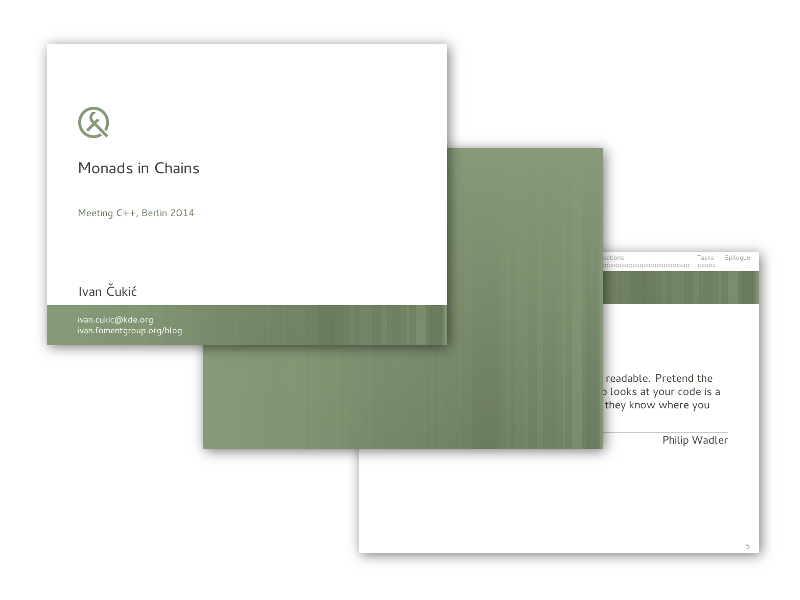
\includegraphics[width=\paperwidth]{../pic/theme-2.png}}
\begin{frame}[plain]
    .
\end{frame}
}


{
\usebackgroundtemplate{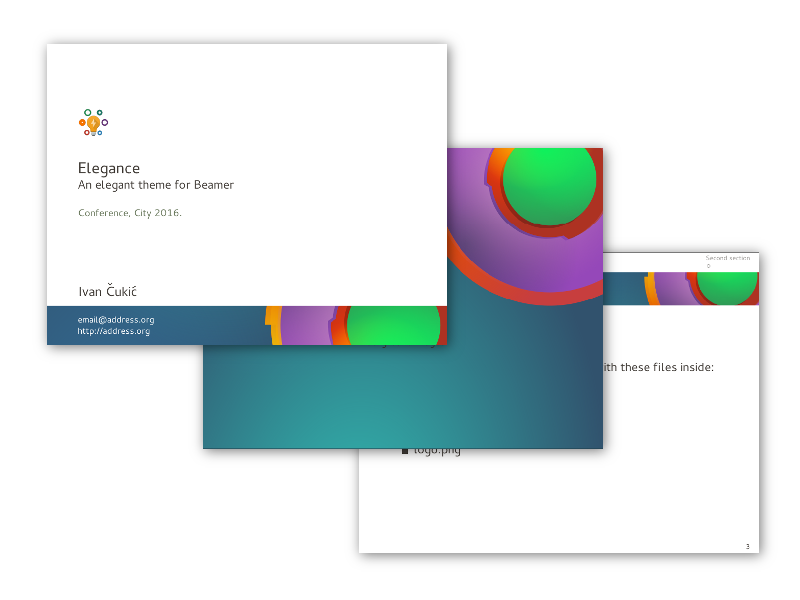
\includegraphics[width=\paperwidth]{../pic/theme-3.png}}
\begin{frame}[plain]
    .
\end{frame}
}





\section{Examples}

\subsection{Showing code}

\begin{xframe}{Code snippets}

    Do you have some code to show on the slide?

    And the same frame should also contain text?

    \begin{cxxcodebox}
        class example {
            // \codedots shows grayed-out dots
            @ \codedots @
        };
    \end{cxxcodebox}

    You can use \verb|cxxcodebox| environment.
    It has \verb|cxx| in the name,
    but no syntax highlighting is performed.

    For short code snippets,
    it is better just to highlight the important parts.

\end{xframe}


\subsection{Code slides and escapes}

\begin{xframe}{Second slide}

    \begin{cxxcode}
        class example {
            // There are a few useful escapes here
            @ \codedots @ // \codedots shows grayed-out dots

            // Invalid parts can be marked with \hlErr
            @\hlErr{operator;}@

            // Good parts can be marked with \hlOk
            @\hlOk{operator() ()}@

            // Other highlighting commands can be seen in
            // the preamble.tex file
        };
    \end{cxxcode}

\end{xframe}

\end{document}
